\documentclass[12pt,letterpaper]{article}
\usepackage{graphicx,textcomp}
\usepackage{natbib}
\usepackage{setspace}
\usepackage{fullpage}
\usepackage{color}
\usepackage[reqno]{amsmath}
\usepackage{amsthm}
\usepackage{fancyvrb}
\usepackage{amssymb,enumerate}
\usepackage[all]{xy}
\usepackage{endnotes}
\usepackage{lscape}
\newtheorem{com}{Comment}
\usepackage{float}
\usepackage{hyperref}
\newtheorem{lem} {Lemma}
\newtheorem{prop}{Proposition}
\newtheorem{thm}{Theorem}
\newtheorem{defn}{Definition}
\newtheorem{cor}{Corollary}
\newtheorem{obs}{Observation}
\usepackage[compact]{titlesec}
\usepackage{dcolumn}
\usepackage{tikz}
\usetikzlibrary{arrows}
\usepackage{multirow}
\usepackage{xcolor}
\newcolumntype{.}{D{.}{.}{-1}}
\newcolumntype{d}[1]{D{.}{.}{#1}}
\definecolor{light-gray}{gray}{0.65}
\usepackage{url}
\usepackage{listings}
\usepackage{color}

\definecolor{codegreen}{rgb}{0,0.6,0}
\definecolor{codegray}{rgb}{0.5,0.5,0.5}
\definecolor{codepurple}{rgb}{0.58,0,0.82}
\definecolor{backcolour}{rgb}{0.95,0.95,0.92}

\lstdefinestyle{mystyle}{
	backgroundcolor=\color{backcolour},   
	commentstyle=\color{codegreen},
	keywordstyle=\color{magenta},
	numberstyle=\tiny\color{codegray},
	stringstyle=\color{codepurple},
	basicstyle=\footnotesize,
	breakatwhitespace=false,         
	breaklines=true,                 
	captionpos=b,                    
	keepspaces=true,                 
	numbers=left,                    
	numbersep=5pt,                  
	showspaces=false,                
	showstringspaces=false,
	showtabs=false,                  
	tabsize=2
}
\lstset{style=mystyle}
\newcommand{\Sref}[1]{Section~\ref{#1}}
\newtheorem{hyp}{Hypothesis}

\title{Problem Set 1}
\date{Due: October 8, 2026}
\author{Applied Stats/Quant Methods 1}

\begin{document}
	\maketitle
	
	\section*{Instructions}
	\begin{itemize}
	\item Please show your work! You may lose points by simply writing in the answer. If the problem requires you to execute commands in \texttt{R}, please include the code you used to get your answers. Please also include the \texttt{.R} file that contains your code. If you are not sure if work needs to be shown for a particular problem, please ask.
\item Your homework should be submitted electronically on GitHub.
\item This problem set is due before 23:59 on Thursday October 8, 2026. No late assignments will be accepted.
	\end{itemize}
	
	\vspace{1cm}
	\section*{Question 1: Education}

A school counselor was curious about the average of IQ of the students in her school and took a random sample of 25 students' IQ scores. The following is the data set:\\
\vspace{.5cm}

\lstinputlisting[language=R, firstline=36, lastline=36]{PS01.R}  


\vspace{1cm}

\begin{enumerate}
	\item Find a 90\% confidence interval for the average student IQ in the school (As a hint, you first need the mean and SD to create a CI):\\
	
	\lstinputlisting[language=R, firstline=37, lastline=71]{PS01.R}  
	
	The sample mean is 98.44, the sample standard deviation is 13.09, and the sample size is 25. Because the population standard deviation is unknown, I use the t-distribution with df=n-1=24.
	
	For a 90\% confidence interval, alpha=0.10, so the t value is 1.71. The standard error is 2.619, and the margin of error is 4.48. Therefore, the confidence interval is 93.96 to 102.92.
	
	So, I am 90\% confident that the mean IQ of students at this school lies between 93.96 and 102.92.
	
	
	\item Next, the school counselor was curious  whether  the average student IQ in her school is higher than the average IQ score (100) among all the schools in the country.\\ 
	
	\noindent Using the same sample, conduct the appropriate hypothesis test with $\alpha=0.05$.
	
	\lstinputlisting[language=R, firstline=73, lastline=84]{PS01.R}  
	
	The null hypothesis is that average student IQ in her school = 100, and alternative hypothesis is that it's greater than 100. This is a one-sided t-test. The test statistic is taken by comparing the sample mean to 100 and then dividing by standard error to get -0.596. Then using 24 degrees of freedom, the one-sided p-value is 0.722. 
	
	Since p=0.722 is greater than alpha=0.05, I fail to reject the null hypothesis. There is insufficient evidence at the 5\% significance level to conclude that the mean IQ of students
	at this school is greater than 100.
	
\end{enumerate}

\newpage

	\section*{Question 2: Political Economy}

\noindent Researchers are curious about what affects the amount of money communities spend on addressing homelessness. The following variables constitute our data set about social welfare expenditures in the USA. \\
\vspace{.5cm}


\begin{tabular}{r|l}
	\texttt{State} &\emph{50 states in US} \\
	\texttt{Y} & \emph{per capita expenditure on shelters/housing assistance in state}\\
	\texttt{X1} &\emph{per capita personal income in state} \\
	\texttt{X2} &  \emph{Number of residents per 100,000 that are "financially insecure" in state}\\
	\texttt{X3} &  \emph{Number of people per thousand residing in urban areas in state} \\
	\texttt{Region} &  \emph{1=Northeast, 2= North Central, 3= South, 4=West} \\
\end{tabular}

\vspace{.5cm}
\noindent Explore the \texttt{expenditure} data set and import data into \texttt{R}.
\vspace{.5cm}
\lstinputlisting[language=R, firstline=88, lastline=88]{PS01.R}  
\vspace{.5cm}
\lstinputlisting[language=R, firstline=90, lastline=93]{PS01.R} 
\begin{itemize}

\item
Please plot the relationships among \emph{Y}, \emph{X1}, \emph{X2}, and \emph{X3}? What are the correlations among them (you just need to describe the graph and the relationships among them)?
\vspace{.5cm}
\lstinputlisting[language=R, firstline=95, lastline=101]{PS01.R}  
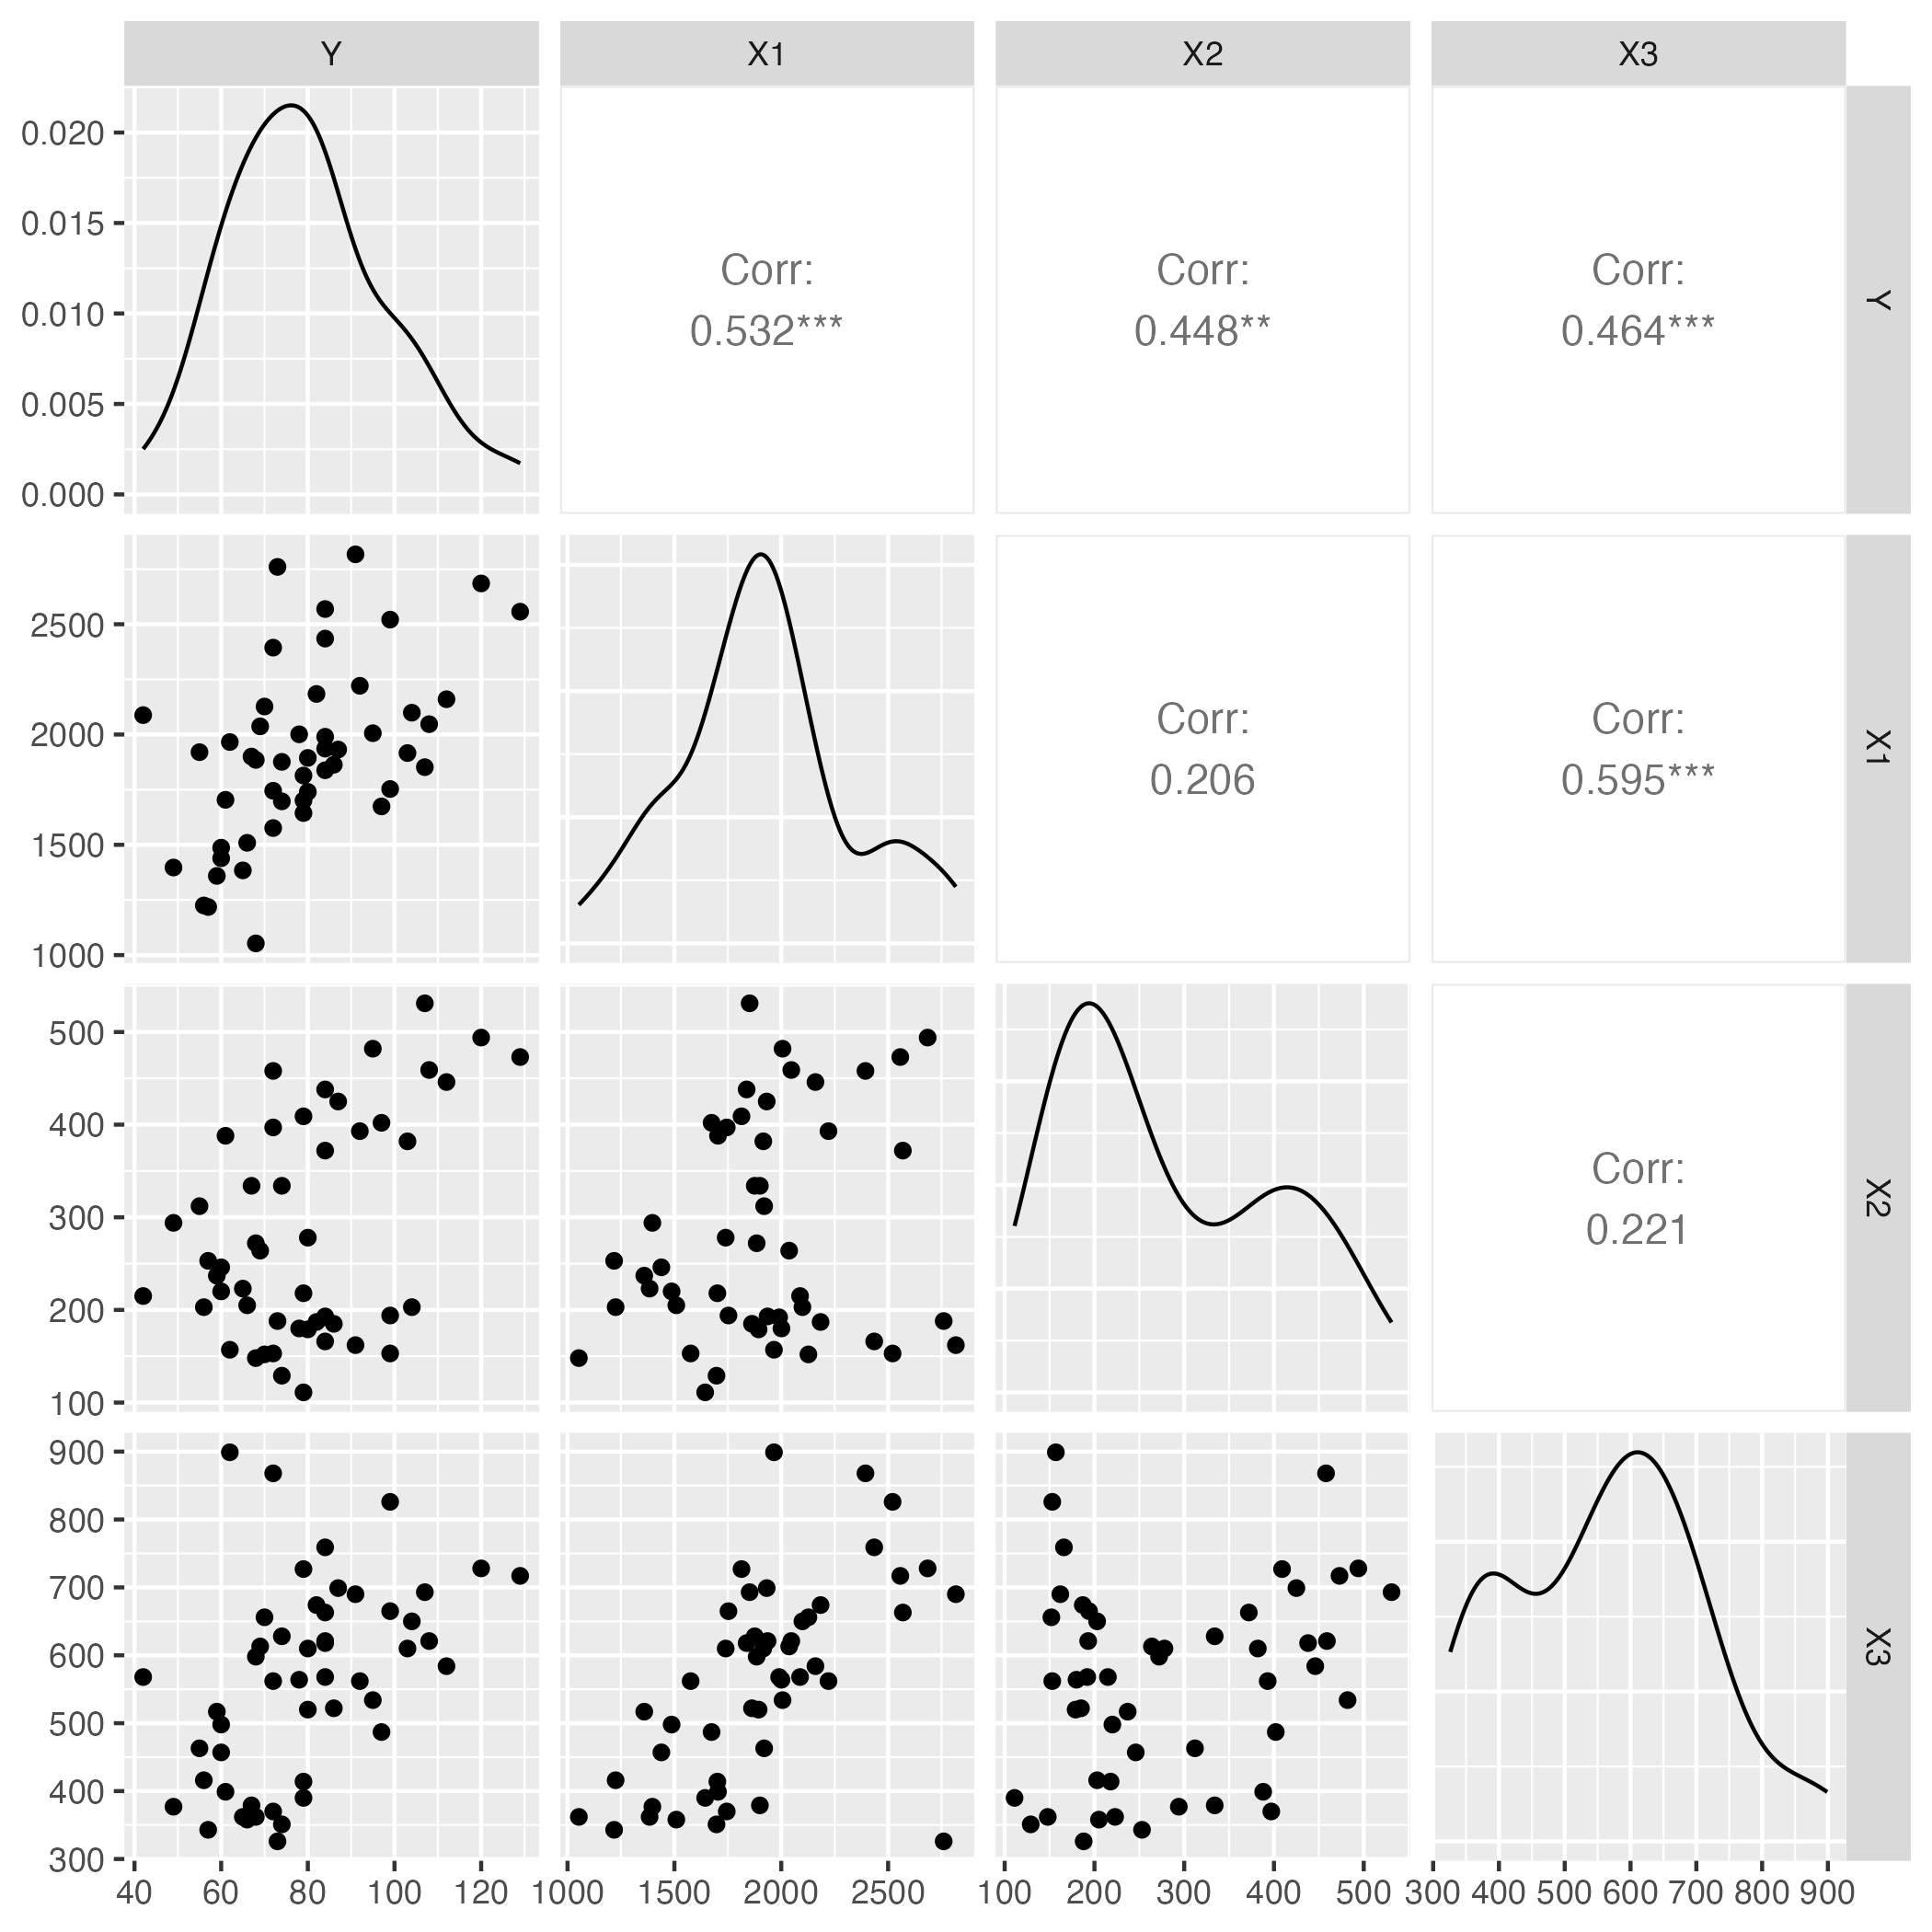
\includegraphics[width=0.8\textwidth]{graph_1.png}

The scatterplots show positive relationships between all four variables. Y (per capita expenditure on housing assistance) has moderate positive relationships with X1 (per capita personal income) (0.532), X2 (the number of financially insecure residents per 100,000) (0.448), and X3 (the number of people per 1,000 in urban areas) (0.464). This means that higher values of each of these variables generally correspond with higher housing expenditures, although there is substantial variation. The strongest relationship is between X1 and X3, with a correlation of 0.595, suggesting that states with higher per capita personal income also tend to have a larger share of their population living in urban areas. The relationships between X1 and X2 (0.206) and between X2 and X3 (0.221) are comparatively weak. Overall, all of the relationships are positive, but none are especially strong, and the graphs show considerable spread around these general patterns.

\item
Please plot the relationship between \emph{Y} and \emph{Region}? On average, which region has the highest per capita expenditure on housing assistance?
\vspace{.5cm}
\lstinputlisting[language=R, firstline=105, lastline=135]{PS01.R}
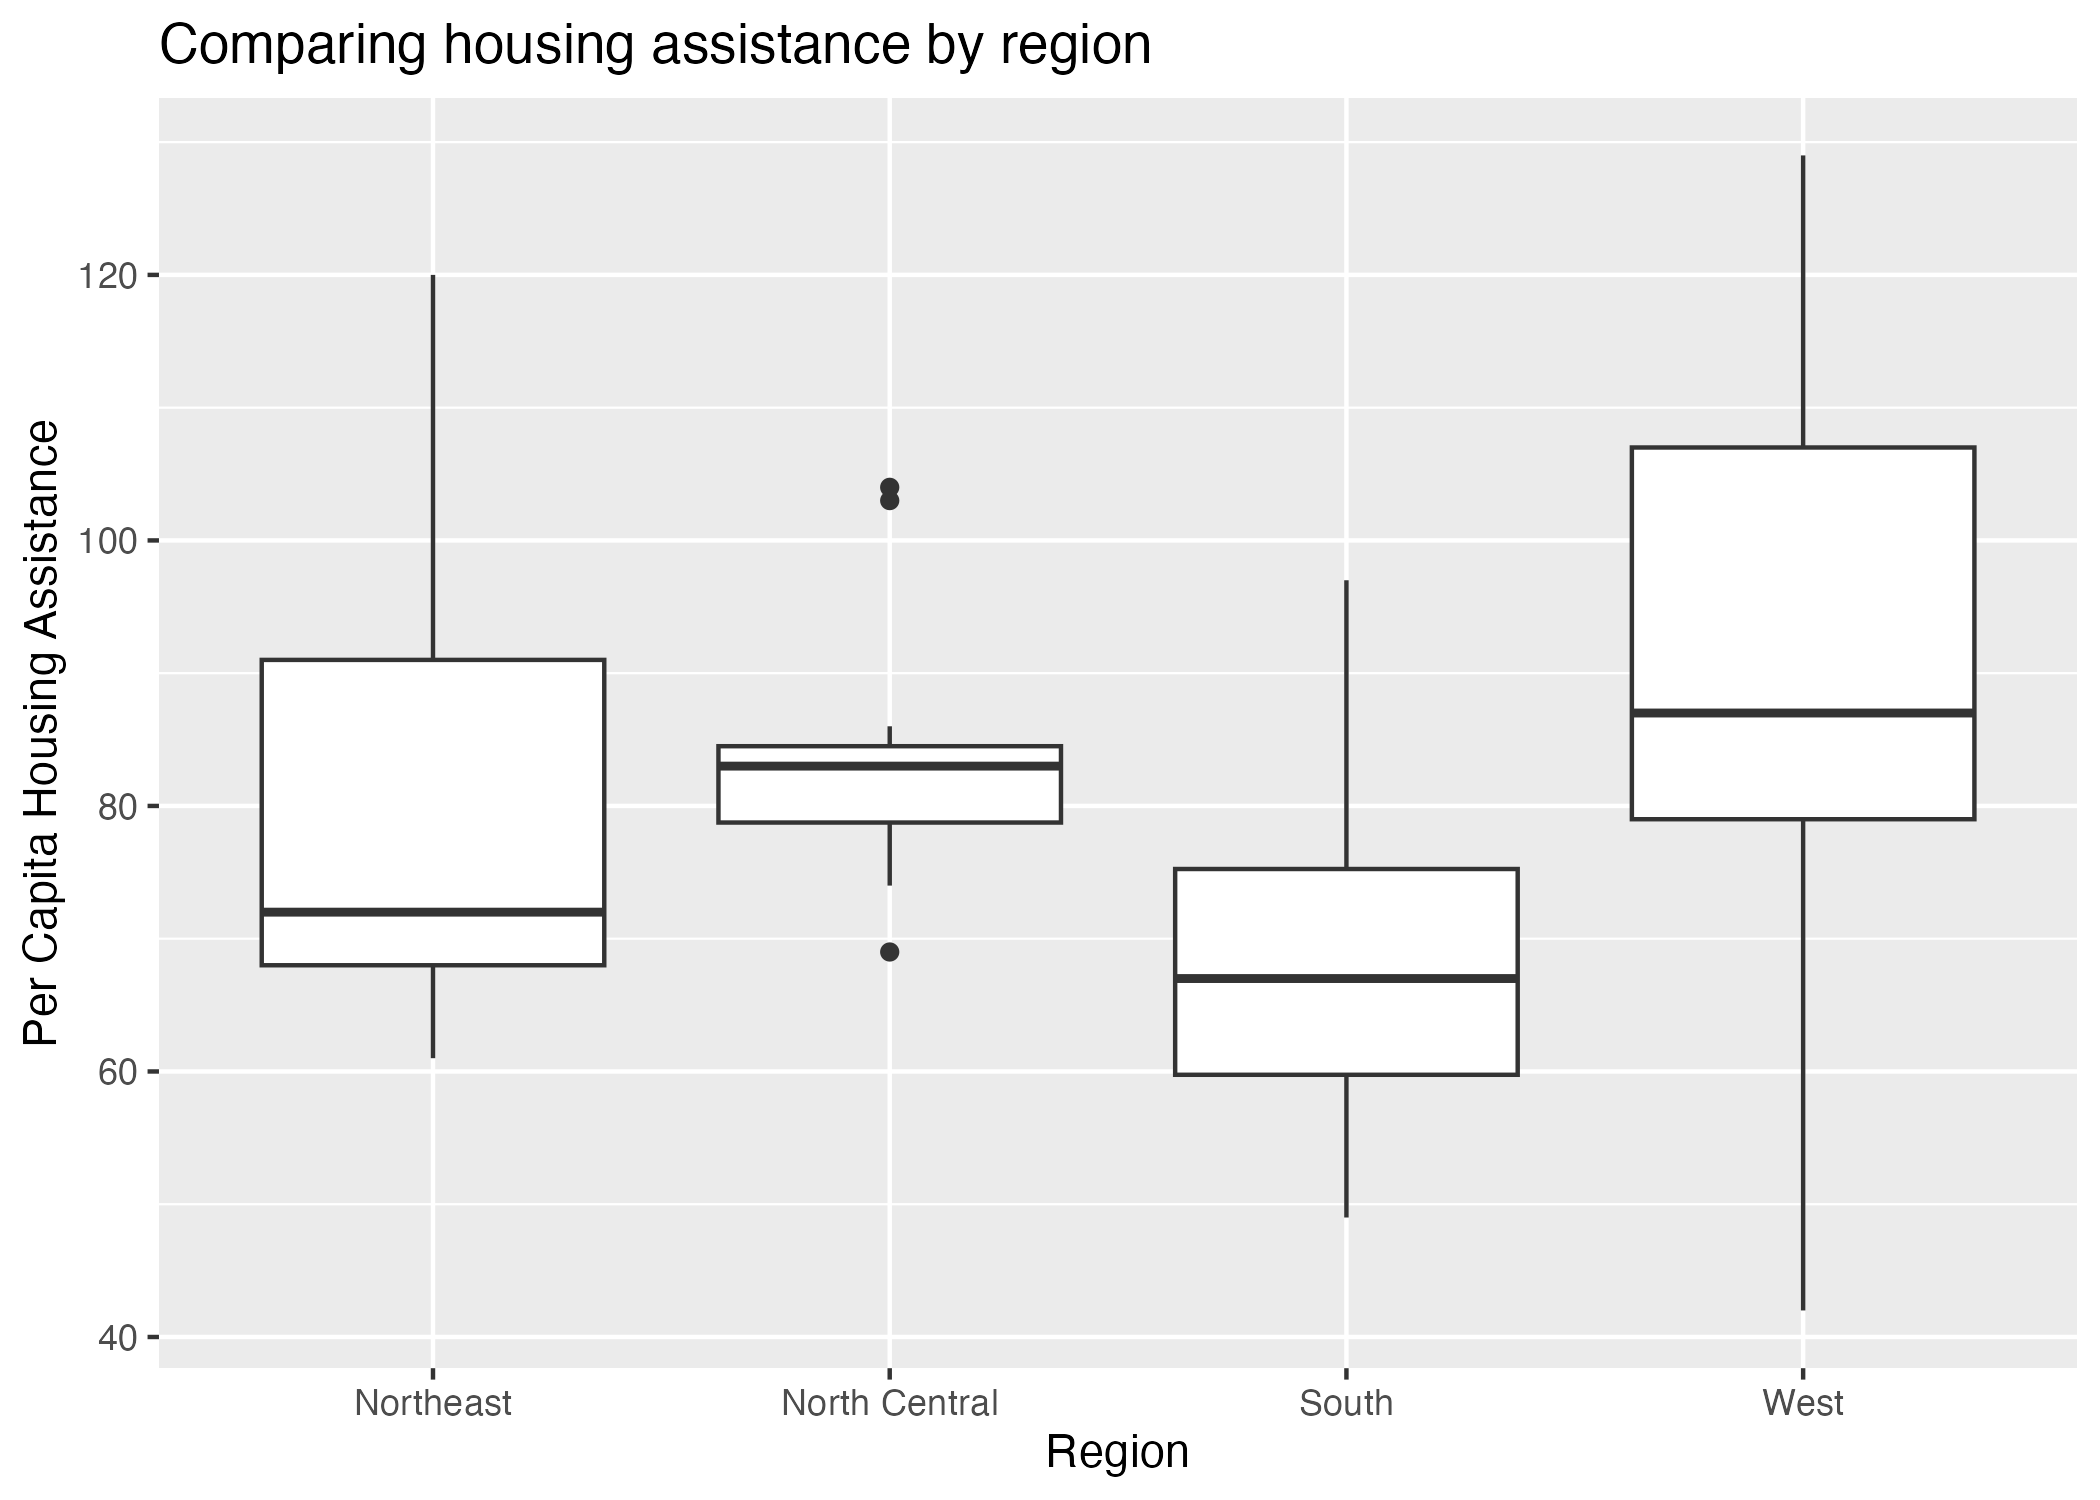
\includegraphics[width=0.8\textwidth]{graph_y_region.png}

The boxplot shows differences in housing assistance expenditure across the four regions, although there is also variation within each region. The South generally has lower expenditures, while the West and North Central regions tend to have higher expenditures.

 The mean per capita expenditure on housing assistance is approximately 79.4 in the Northeast, 83.9 in North Central, 69.2 in the South, and 88.3 in the West. Therefore, the West has the highest average per capita expenditure on housing assistance, with a mean of approximately 88.3.
 
\item
Please plot the relationship between \emph{Y} and \emph{X1}? Describe this graph and the relationship. Reproduce the above graph including one more variable \emph{Region} and display different regions with different types of symbols and colors.
\lstinputlisting[language=R, firstline=137, lastline=148]{PS01.R}
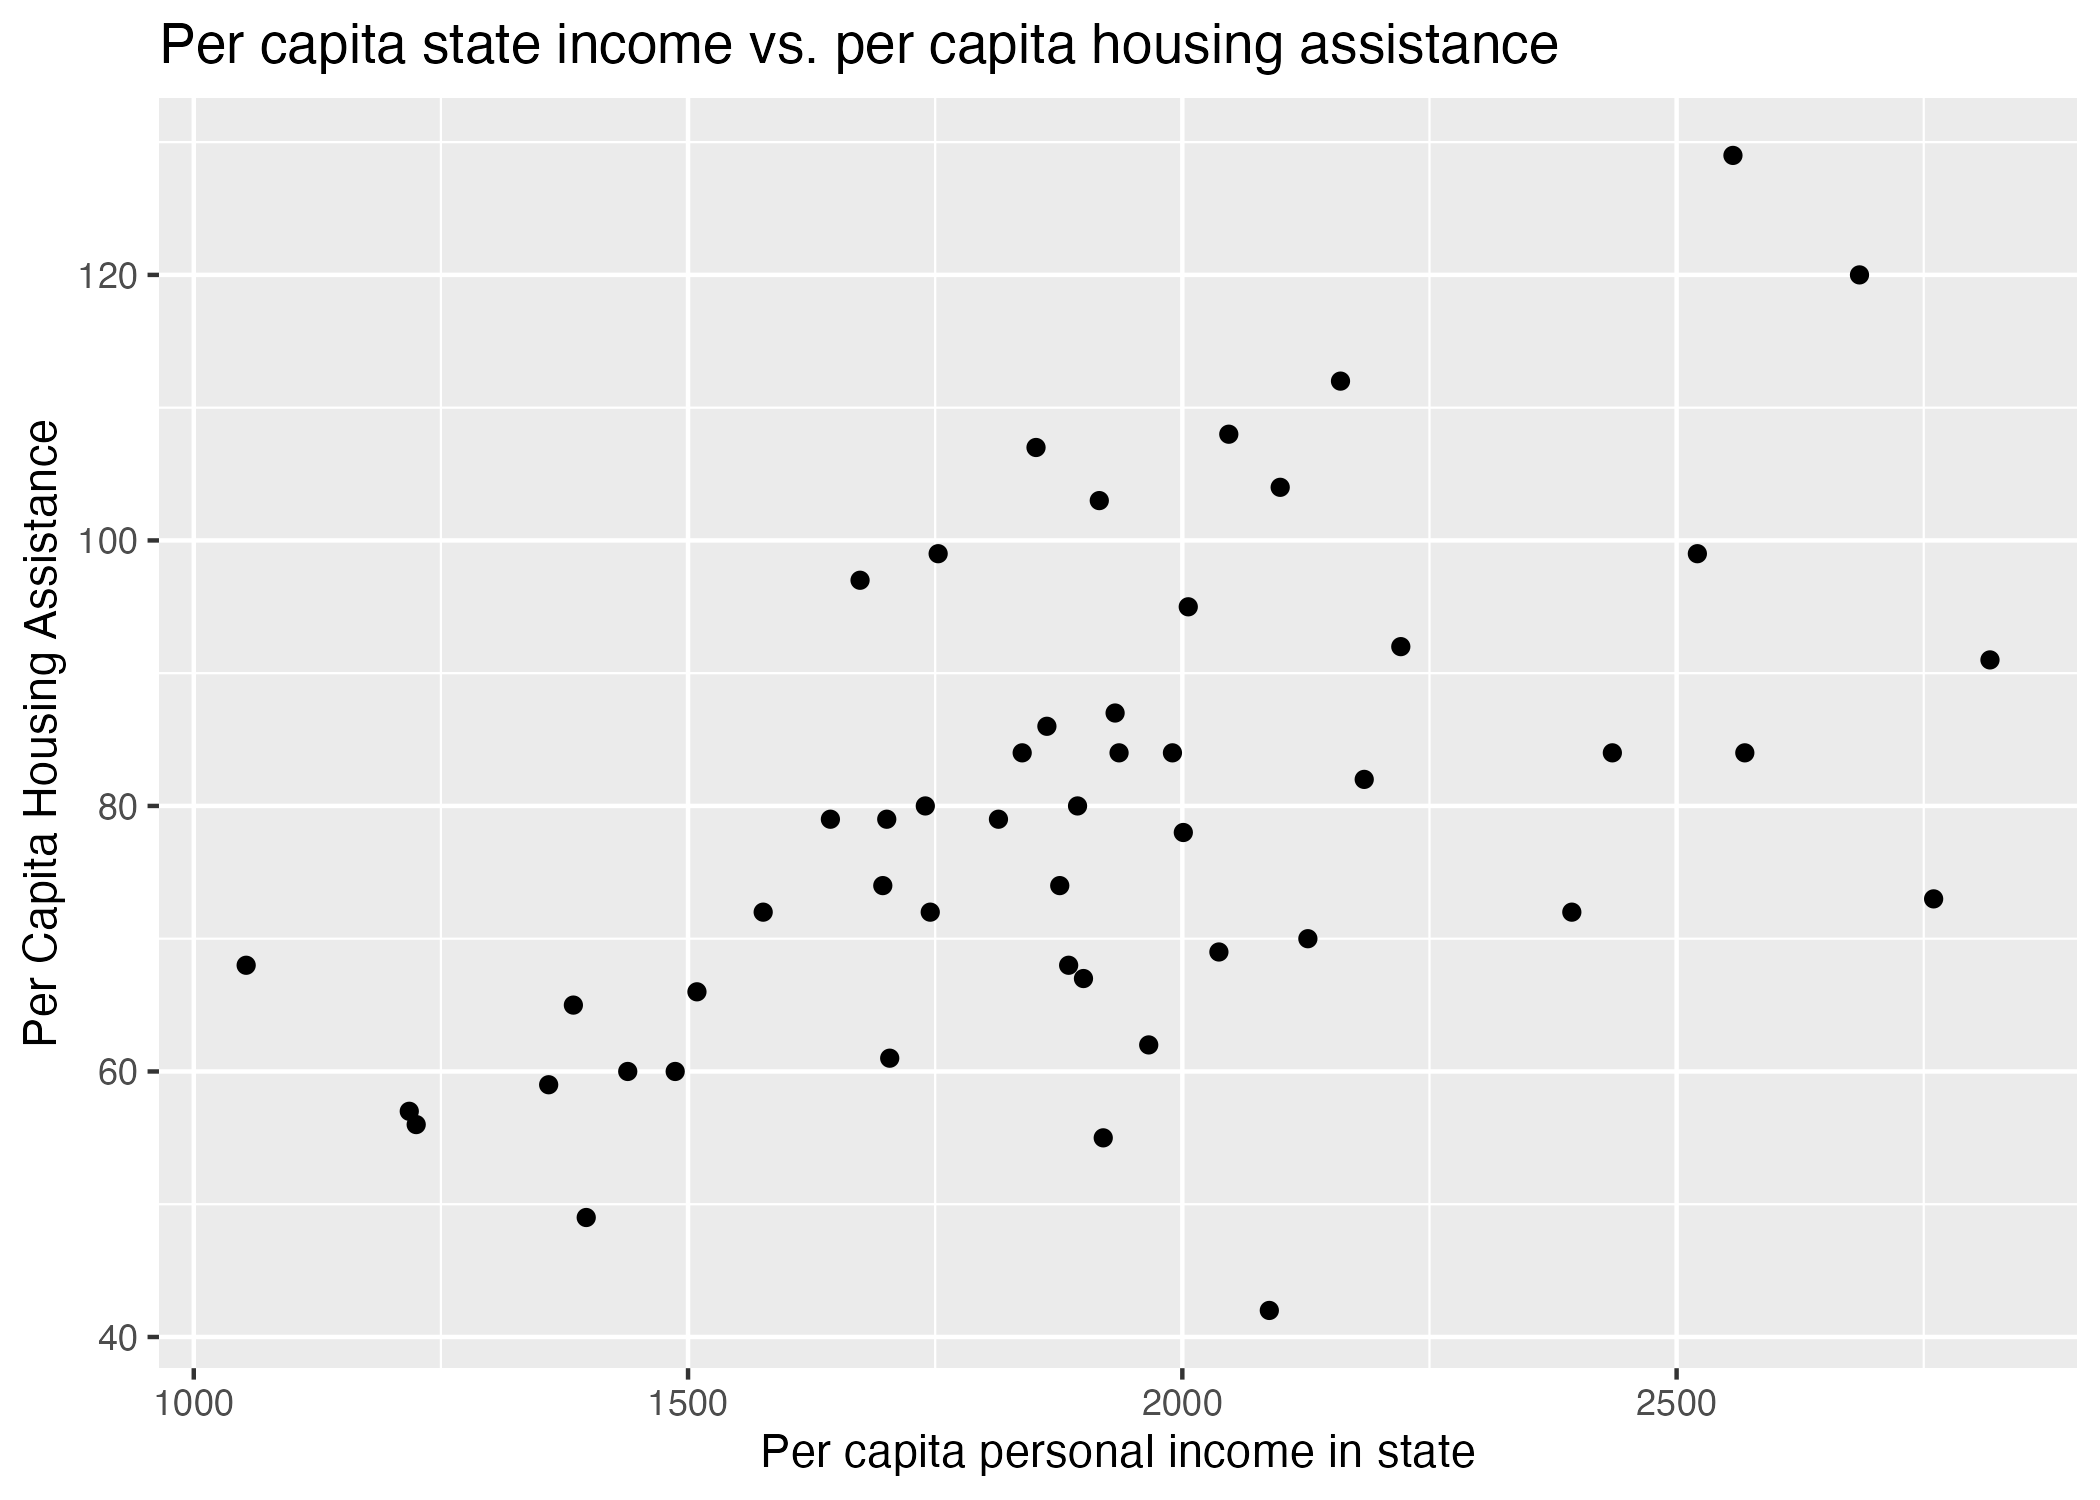
\includegraphics[width=0.8\textwidth]{graph_y_X1.png}

The scatterplot shows a moderate positive relationship between per capita personal income (X1) and per capita expenditure on housing assistance (Y). States with higher personal income generally tend to have higher housing assistance expenditures, although the points are fairly spread out, so the relationship is not especially strong.
\lstinputlisting[language=R, firstline=152, lastline=163]{PS01.R}
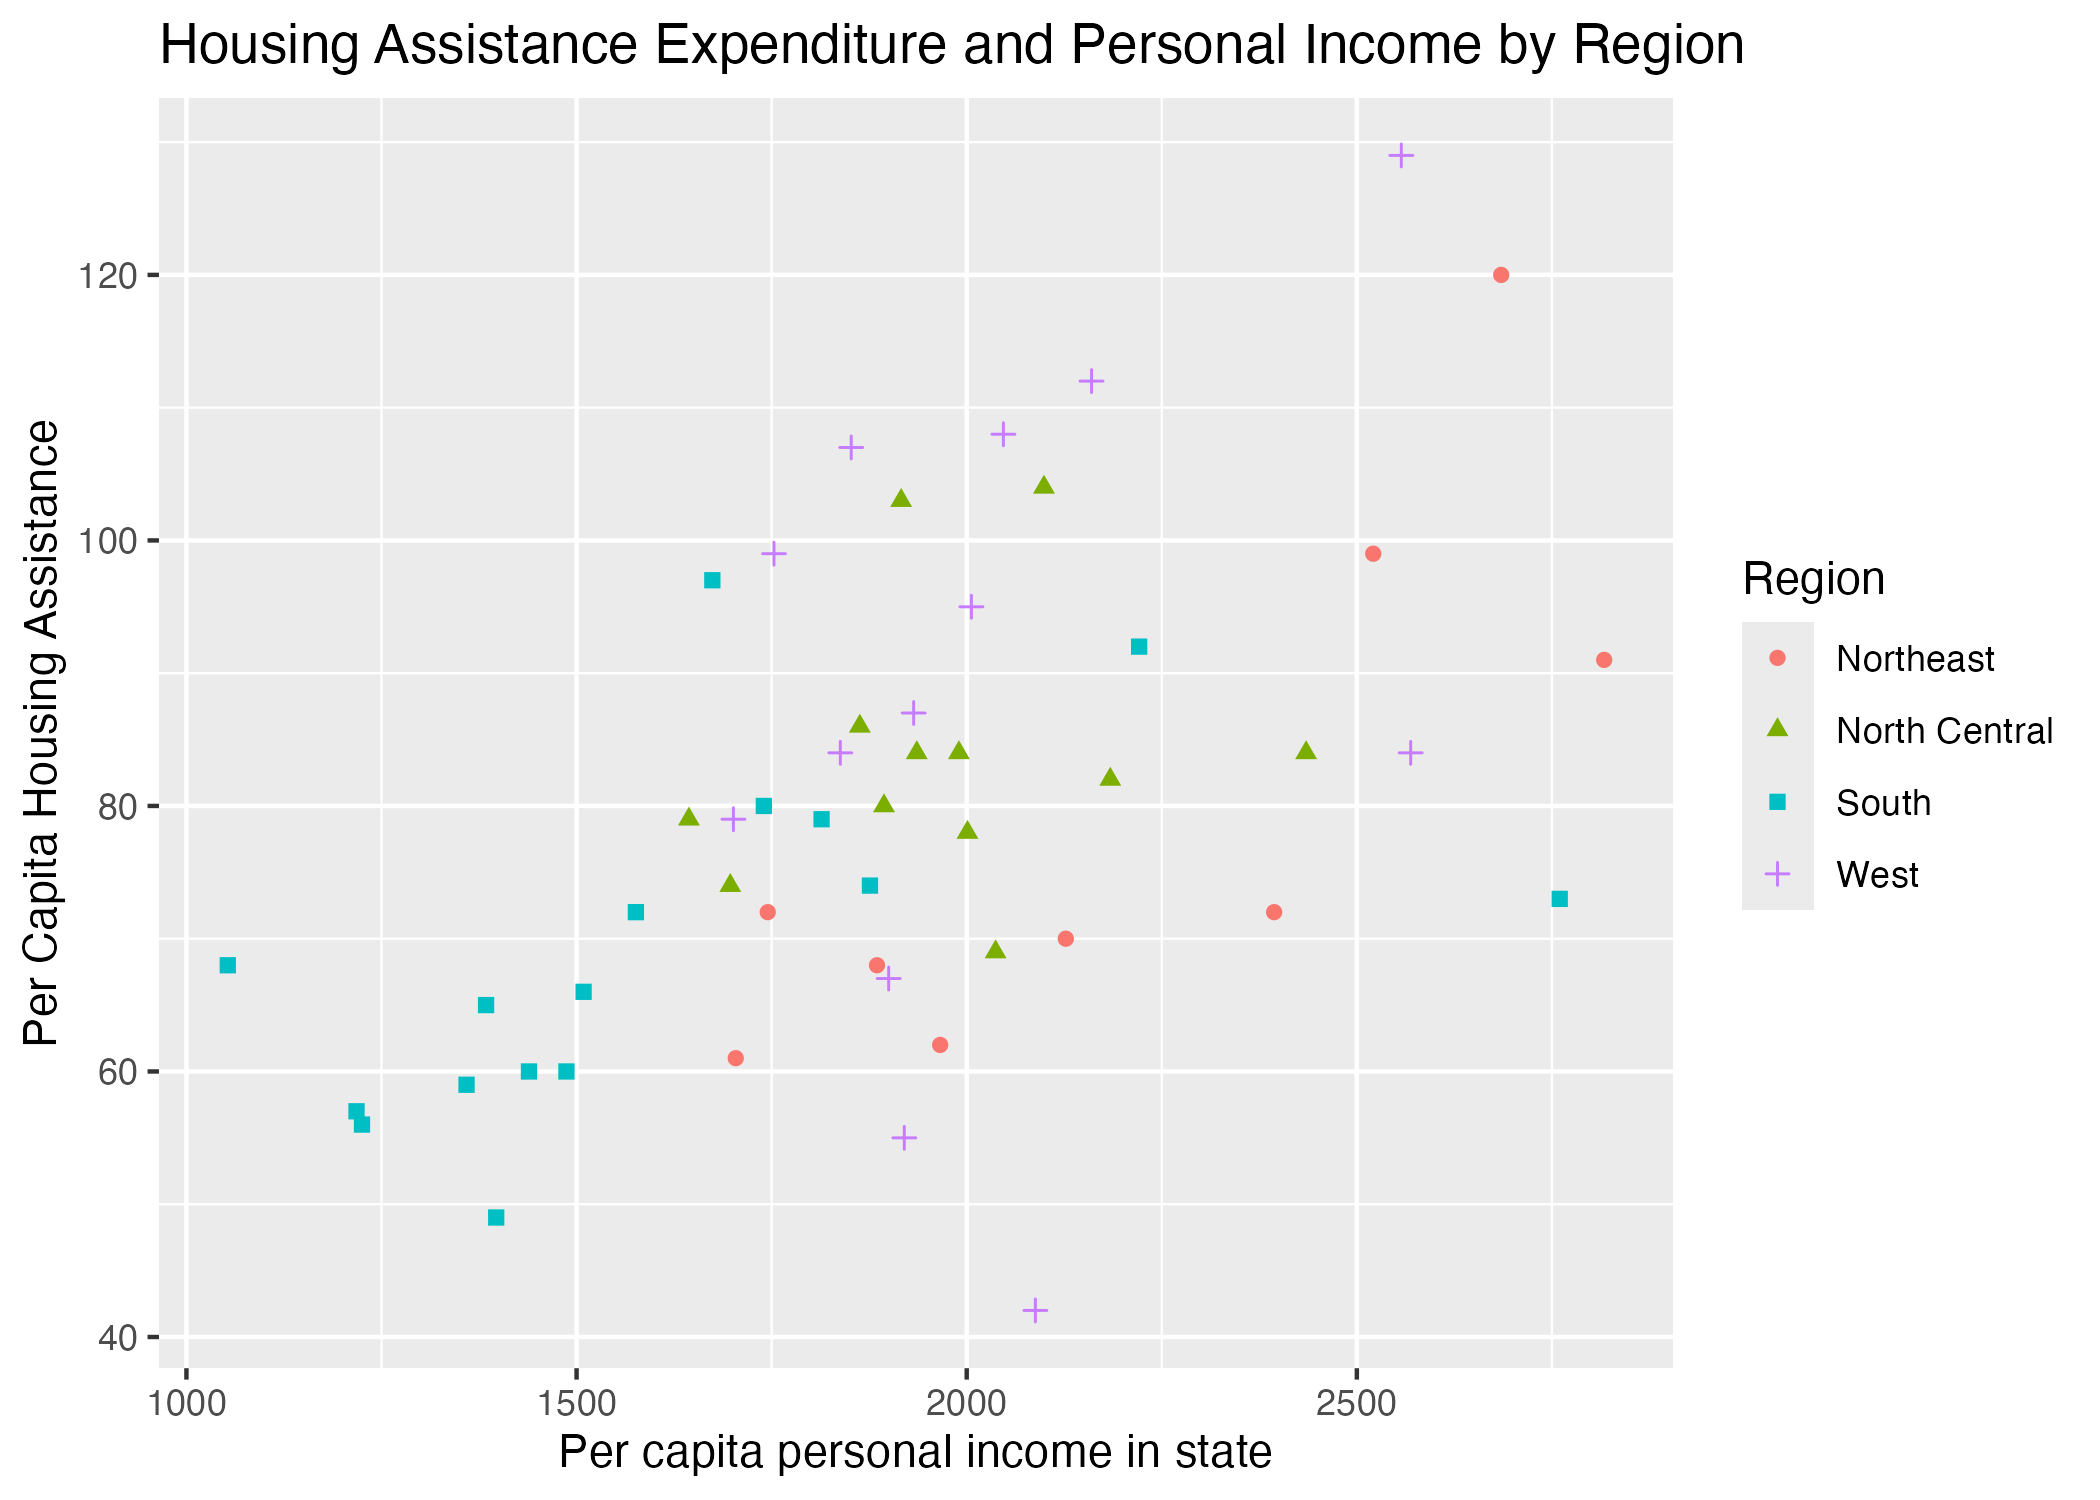
\includegraphics[width=0.8\textwidth]{graph_y_X1_region.png}
\end{itemize}


\end{document}
